\documentclass[border=10pt]{standalone}
\usepackage{pgfplots}
\pgfplotsset{compat=1.18}
\usepgfplotslibrary{colormaps}

\begin{document}
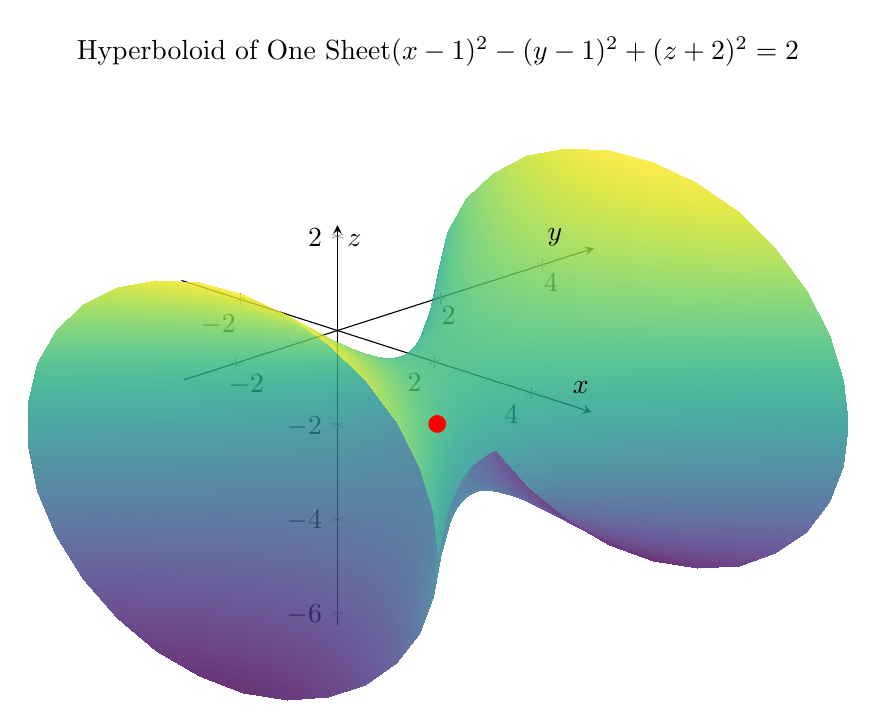
\begin{tikzpicture}
\begin{axis}[
    width=12cm,
    height=10cm,
    xlabel={$x$},
    ylabel={$y$},
    zlabel={$z$},
    title={Hyperboloid of One Sheet \\ $(x-1)^2 - (y-1)^2 + (z+2)^2 = 2$},
    view={45}{25},
    colormap/viridis,
    grid=major,
    axis lines=center,
    ]
    
    % Plot the hyperboloid of one sheet
    % Parametric form: x = 1 + sqrt(2+(y-1)^2)*cos(theta), z = -2 + sqrt(2+(y-1)^2)*sin(theta)
    \addplot3[
        surf,
        domain=-3:5,
        y domain=0:360,
        samples=30,
        samples y=30,
        opacity=0.8,
        shader=interp,
    ]
    ({1 + sqrt(2+(x-1)^2)*cos(y)}, {x}, {-2 + sqrt(2+(x-1)^2)*sin(y)});
    
    % Add center point
    \addplot3[red, only marks, mark=*, mark size=3pt] coordinates {(1,1,-2)};
    
\end{axis}
\end{tikzpicture}
\end{document}